\chapter{Background}
\label{cha:background}

In this chapter, we provide background on some of the topics we study in the
thesis. We begin by describing the \acf{CA} model, which is the complex system
we focus on in most of the thesis (Section \ref{sec:cellular-automata-sec}).
Next, we describe the similarities between \acp{CA} and \acfp{RNN}, which is
useful for understanding the characteristics and applications these two models
share (Section \ref{sec:cell-autom-rnns}). \acp{CA} can be reformulated
completely as a special case of \acp{RNN}. With this reformulation, using
\acp{CA} as a replacement of \acp{RNN} becomes natural for several use cases. We
describe the \acf{RC} model (Section \ref{sec:res-models}), which enables
sending inputs to, and harvesting the computations of complex systems to solve
problems, which we apply in Chapter~\ref{cha:learn-effic-compl}. This model was
developed with \acp{RNN} but we describe how \acp{CA} and other complex systems
can be a suitable replacement and the benefits of this approach.

\section{Cellular automata}\label{sec:cellular-automata-sec}

The \acf{CA} model was simultaneously proposed by Stanislaw Ulam and John Von
Neumann in the 1940s as a model of the growth of crystals and an attempt at
constructing an autonomously self-replicating system
\parencite{vonneumannTheorySelfreproducingAutomata1966}.

\subsection{Definition}\label{sec:definition}
It is usually defined on a regular lattice in one or two dimensions. Each of its
components is called a cell and can be in a state $k \in \mathcal{S}$. $\mathcal{S}$ is the space of
available states for cells, usually chosen to be $\{0, 1\}$ for binary
\acp{CA} or $\{1, \ldots, n\}$ for \acp{CA} with $n$ states.

A neighborhood function $\boldsymbol{N}$ is defined that associates each cell
with its neighbors on the grid. In general, a \ac{CA} can be constructed on any
space $\mathcal{L}$ where this function can be defined. The space $\mathcal{L}$ specifies an
indexing and the relation between the cells. In practice, regular finite or
infinite grids are chosen, $\mathcal{L} \subset \mathbb{Z}$ or $\mathcal{L} \subset \mathbb{Z}^{2}$. For example, the grid could
be a 1 dimensional torus with 10 cells, that is,
$\mathcal{L}_{{T_{10}}} = \{1, 2, \ldots, 10 \}$. The neighborhood function has the following
general form:
\begin{equation}
  \begin{aligned}
\boldsymbol{N}_{\mathcal{L}} :\quad & \mathcal{S} \rightarrow \mathcal{S}^{s}\\
&c_{i} \mapsto [c_{j}]_{j\in \mathcal{N}_{c_{i}}},
  \end{aligned}
\end{equation}
where $\mathcal{N}_{c_{i}}$ is the neighborhood of cell $c_{i}$, $s$ is the
number of cells in the neighborhood and the returned value is a finite set of
cells: the neighbors of cell $c_{i}$. For the torus $\mathcal{L}_{T_{10}}$
above, we can define the neighbors to be the cell itself and the two immediately
adjacent cells. This type of 1D neighborhood is usually associated with a
\emph{radius} parameter $r = 1$. The $r=1$ neighborhood is illustrated in Figure
\ref{fig:1d_neigh}. It corresponds to the following neighborhood function:
\begin{equation}
  \begin{aligned}
\boldsymbol{N}_{\mathcal{L}_{T_{10}}} :\quad & \mathcal{S} \rightarrow \mathcal{S}^{3} \\
&\boldsymbol{N}_{\mathcal{L}_{T_{10}}}(c_{i}) = \begin{cases}
                      [c_{i - 1}, c_{i}, c_{i + 1}],& \text{if}\quad i \in \{2,\ldots , 9\}\\
                       [c_{10}, c_{1}, c_{2}], & \text{if} \quad i = 1 \\
                       [c_{9}, c_{10}, c_{1}], & \text{if} \quad i = 10. \\
                    \end{cases}
  \end{aligned}
  \label{eq:torus_index}
\end{equation}

A larger radius $r$ would correspond to including more cells in the
neighborhood, going in each direction from the initial cell. On two dimensional
grids, there are multiple ways to define the neighborhood. Some common examples
are the Moore neighborhood (see Figure \ref{fig:moore}) and the Von Neumann
neighborhood (see Figure \ref{fig:von_neumann}). In the rest we omit the
subscript on the neighborhood function $\boldsymbol{N}$ as we almost always work
with regular grids on a torus, for which it is simpler to just mention the size
and dimension.

\begin{figure}[htbp]
  \centering
  \begin{subfigure}[c]{.3\linewidth}
    \centering
    
\includegraphics[width=\linewidth]{figures/1d_neigh}
    \caption{Standard 1D \ac{CA} neighborhood}
    \label{fig:1d_neigh}
  \end{subfigure}
  \begin{subfigure}[c]{.3\linewidth}
    \centering
    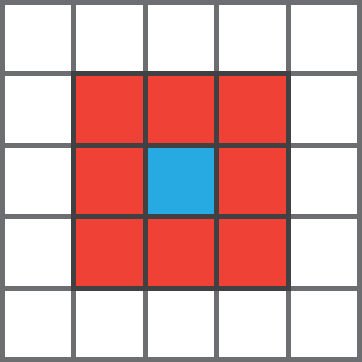
\includegraphics[width=\linewidth]{figures/moore}
    \caption{Moore neighborhood}
    \label{fig:moore}
  \end{subfigure}
  \begin{subfigure}[c]{.3\linewidth}
    \centering
    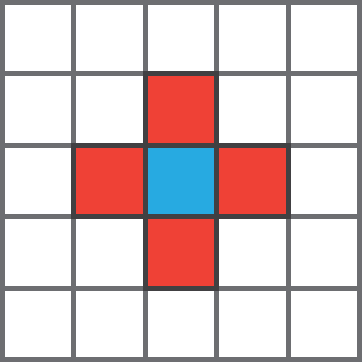
\includegraphics[width=\linewidth]{figures/von_neumann}
    \caption{Von Neumann neighborhood}
    \label{fig:von_neumann}
  \end{subfigure}

  \caption{Illustration of commonly used neighborhoods for 1D and 2D \ac{CA}.}
  \label{fig:neighborhoods}
\end{figure}

A \ac{CA} evolves in discrete time steps. An update rule
$\boldsymbol{\Phi}: \mathcal{S}^{s} \rightarrow \mathcal{S}$ defines the new state of a cell as a
function of its local neighborhood at the current time step. It is applied in
parallel to all cells. For a \ac{CA} in its initial state at time
step 0 --- \ie a set of cells $\left(c_{i}^{(0)}\right)_{i \in \mathcal{L}} \in \mathcal{S}^{|\mathcal{L}|}$, and a
neighborhood function $\boldsymbol{N}$, we have the following update rule:
\begin{equation}
\begin{aligned}
\forall i \in \mathcal{L}, \quad c_{i}^{(t + 1)} = \boldsymbol{\Phi}\left(\boldsymbol{N}\left(c_{i}^{(t)}\right)\right).
\end{aligned}
\end{equation}

The details of an update step in a 1 dimensional \ac{CA} is shown on Figure
\ref{fig:ca_base} for example. The neighborhood of the cell $c_{i}$ is $c_{i}$
itself as well as its two immediately adjacent cells.

\begin{figure}[htbp]
  \centering
 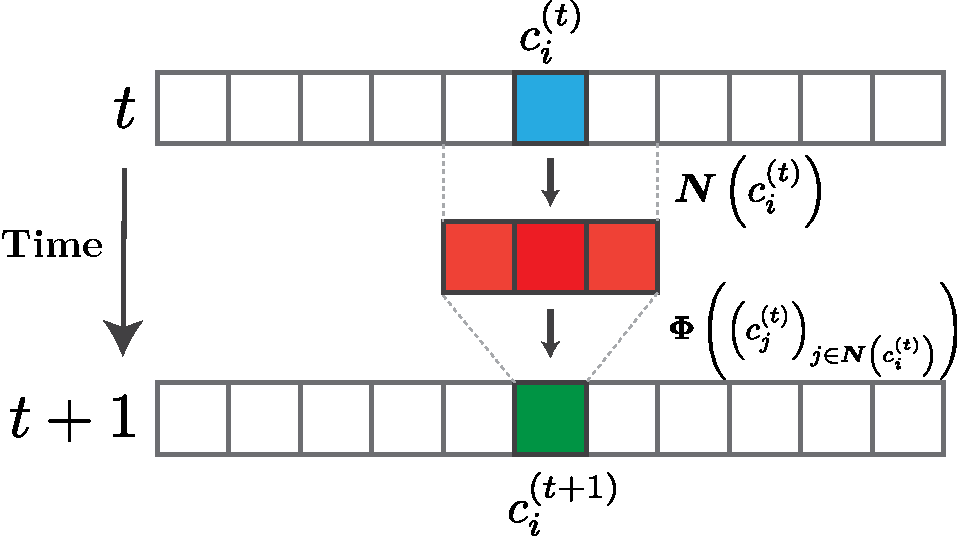
\includegraphics[width=.7\linewidth]{figures/ca_base}
  \caption{Illustration of a \acl{CA} update rule in 1 dimension. For each cell,
  we look up the neighboring cells and update its state according to the current
state of the neighbors.}
  \label{fig:ca_base}
\end{figure}

The function $\boldsymbol{\Phi}$ is often called a \emph{rule table} because it
associates an output state for each possible combination of input neighbor
states. In an implementation of the \ac{CA} model, these output states can be
looked up from a table containing all possible transitions from inputs to
outputs.

\paragraph{Rule representation}
A useful rule representation can be obtained by listing all output states
corresponding to input configurations in a predetermined order. This results in
a list of values $[o_1, \ldots, o_{s^{|\mathcal{S}|}}]$, with $\forall i,\ o_{i} \in \mathcal{S}$, where $s$ is
the number of cells in a neighborhood, $\mathcal{S}$ is the space of available states and
$|\mathcal{S}|$ is the number of available states per cell. Using the $o_{i}$ as the
digits of a base-$|\mathcal{S}|$ number, each rule is uniquely represented by a number.
For example, as explained in more details in Section \ref{sec:elem-cell-autom},
the 256 binary rules in one dimension with neighborhood size 3 can be numbered
from 0 to 255, and are referred to by their number in the literature.

\paragraph{Boundary conditions}
The grid of a \ac{CA} can be finite or infinite. In the infinite case, the grid
is assumed to be initialized to a uniform state, except for a few cells set to
other states. The simulation is then run on these few cells, while the rest of
the infinite grid does not have to be simulated from the start. For a finite
grid, an exhaustive simulation can be run, but one needs to define
boundary conditions. The boundaries can be set to wrap to the other side of the
grid, forming a torus. An example of the corresponding indexing is given in
\eqref{eq:torus_index}. Other choices of boundary condition consists in adding
virtual padding cells outside of the main grid. They can be set to a fixed
state, a randomly chosen state, or mirror the cells on the inside of the grid.
Each of these choices affects the evolution and properties of the \ac{CA}, but
the importance of these boundaries decreases for very large grids.

\subsection{Classification of cellular automata\label{sec:class-cell-autom}}

Stephen Wolfram approached \acp{CA} as discrete, spatially extended dynamical
systems \parencite{wolframUniversalityComplexityCellular1984}. The analogy is
only superficial since many concepts from dynamical systems theory, such as
``chaos'', ``attractors'' and ``sensitivity to initial conditions'' only admit a
rigourous definition in the continuous state and continuous time models. Wolfram
proposed a qualitative classification of CA behavior roughly analogous to
classifications in dynamical systems theory, with four classes defined as
follows:

\begin{description}
  \item[Class 1] All initial configurations relax after a transient
        period to the same fixed configuration (e.g., all 1s).
  \item[Class 2] All initial configurations relax after a transient period to some
        fixed point or some temporally periodic cycle of configurations, but
        which one depends on the initial configuration. (\ac{CA} defined on
        finite lattices always end up having a periodic behavior because there
        is only a finite number of grid configurations. Class 2 does not refer to
        this type of periodic behavior but rather to cycles with periods much
        shorter than the total number of possible states).
  \item[Class 3] All initial configurations quickly exhibit chaotic behavior
        after a transient period. (The term “chaotic” here refers to
        apparently unpredictable space-time behavior.)
  \item[Class 4] Some initial configurations result in complex localized
        structures that can persist for a long time.
\end{description}

This classification being qualitative and not rigorous, there is not even a
clear consensus on which of the \acp{ECA} rules belong to class 4 or class 3.
Class 4 \ac{CA} rules are speculated to be capable of universal computation
\parencite{wolframUniversalityComplexityCellular1984}. For example,
\textcite{liStructureElementaryCellular1990} claimed that \ac{ECA} rule 110 has
class 4 behavior, and it was eventually proven to be universal
\parencite{cookUniversalityElementaryCellular2004}, but no other \ac{ECA} has
been proven universal since.

\textcite{zenilCompressionBasedInvestigationDynamical2010} studied the
compression size of the space-time diagrams of all \ac{ECA} for a fixed-length
simulation. Using a simple k-means clustering technique, he obtained two groups
roughly matching Wolfram’s classes 1 and 2 and classes 3 and 4. We reproduce
these results on figure \ref{subfig:comp_scores}. They offer an interesting
non-qualitative confirmation of the results of Wolfram's classification.
However, these results vary significantly if we modify the initial conditions as
well as the grid size, data representation, or compression algorithm
\parencite{hudcovaClassificationComplexSystems2020}.

\textcite{wuenscheGlobalDynamicsCellular1992} studied the behavior of \acp{ECA}
when the simulations are reversed and compute the preimages of each
configuration. They introduced the Z-parameter, which is the probability that a
partial preimage can be extended by one symbol for each \ac{CA}. He speculates
that class 4 occurs at $\text{Z} \approx 0.75$. This is not a classification, but a
class 4 membership test that can be computed from the rule directly, making it
practical compared to alternatives. However when tested in practice, Wuensche's
hypothesis that $\text{Z} \approx 0.75$ corresponds to class 4 is rarely verified.

Hudcová defined a \ac{CA} classification that is based on the form of the
asymptotic growth of their transients, obtained through repeated simulation of
\ac{CA} rules starting from various initial conditions and using the best
fitting function for the asymptotic growth of its transients
\parencite{hudcovaClassificationComplexSystems2020,
  hudcovaClassificationDiscreteDynamical2022}.

\subsection{Cellular automata variants}

A large number of \acp{CA} variants have been proposed, modifying or
constraining various parts of the definition in Section \ref{sec:definition}.
We list some common ones here.

\paragraph{Elementary cellular automata.\label{sec:elem-cell-autom}}
\Acp{ECA} are the 1 dimensional \acp{CA} with two states per cell and
neighborhood size 3 --- the cell and its two direct neighbors on the 1D grid.
There are 8 possible configurations of a neighborhood with 3 cells and 2 states
per cell, which corresponds to 256 possible ways to define an \ac{ECA} --- two
possible outputs for each of these 8 possible configurations; hence
$2^{8} = 256$ possible \ac{CA}. This relatively small number of rules enables
exhaustive exploration of the rule space and mapping of the properties of \ac{ECA},
which would not be possible for general \acp{CA}.

\begin{figure}[htbp]
  \centering
  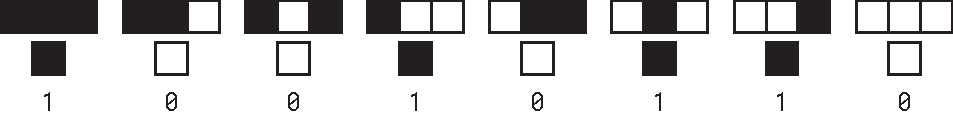
\includegraphics[width=.95\linewidth]{figures/eca_150_rule}
  \caption{Illustration of the rule of \ac{ECA} number 150.}
  \label{fig:eca_150_rule}
\end{figure}

These \acp{CA} are studied extensively, and offer an interesting combination of
trivial definition and implementation and complex and unpredictable properties.
One of the fundamental problems of \ac{CA} research is to classify the 256 rules
into well-defined behavior types and order them by complexity, which was
attempted in several previous works
\parencite{wuenscheGlobalDynamicsCellular1992,
  gutowitzTransientsCyclesComplexity1991,
  wuenscheClassifyingCellularAutomata1999, wolframNewKindScience2002,
  zenilCompressionBasedInvestigationDynamical2010,
  hudcovaClassificationComplexSystems2020,
  hudcovaComputationalHierarchyElementary2021}. We discuss these classifications
in more details in section \ref{sec:class-cell-autom}.

\begin{figure}[htbp]
  \centering
\begin{subfigure}[b]{.45\linewidth}
  \centering
  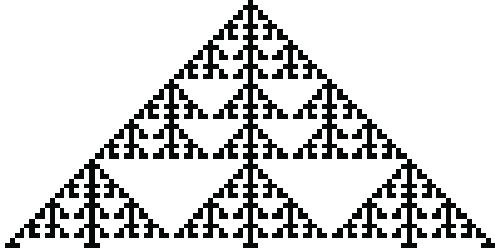
\includegraphics[width=\linewidth]{figures/eca_150_single.pdf}
  \caption{Single cell initialization}
  \label{fig:eca_150_single}
\end{subfigure}
\begin{subfigure}[b]{.45\linewidth}
  \centering
  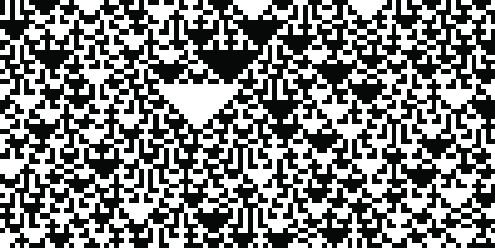
\includegraphics[width=\linewidth]{figures/eca_150_random.pdf}
  \caption{Random initialization}
  \label{fig:eca_150_random}
\end{subfigure}
\caption{Evolution of \ac{ECA} number 150 simulated on a grid of size 100 for 50
  steps. \ref{fig:eca_150_single} shows a simulation starting from a blank grid
  with only one cell set to 1. \ref{fig:eca_150_random} shows a simulation
  starting from a random initialization.}
  \label{fig:eca_150}
\end{figure}


\ac{ECA} rules are easily visualized because there are only 8 possible
neighborhood configurations that need to be shown. For example, figure
\ref{fig:eca_150_rule} shows the transition table for \ac{ECA} rule 150. If we
assign 1 to the black state and 0 to the white state, the possible neighborhood
configurations are ordered in their binary order from right to left, with the
leftmost bit being the most significant one. This is how the rule number is
computed, using the output states (last row in figure \ref{fig:eca_150_rule}) as
a binary representation.

There are several well known \ac{ECA} rules with particularly interesting
properties. For example, a universal computer has been constructed in rule 110
\parencite{cookUniversalityElementaryCellular2004}, making it the first (and
only so far) Turing complete \ac{ECA}.

\paragraph{Totalistic cellular automata.}
Totalistic \ac{CA} are a subset of \ac{CA} which rules can be expressed as a
function of the sum of neighboring cell values. These \ac{CA} were introduced by
Stephen Wolfram \parencite{wolframStatisticalMechanicsCellular1983}. For
example, \ac{ECA} 150 which rule is shown in figure \ref{fig:eca_150_rule} is a
totalistic \ac{CA}. Its rule could be summarized as ``if exactly two states are
1 or all states are 0, the next state is 0, otherwise if one or three states are
1, the next state is 1''. Conway's Game of Life, presented in the following paragraph, is an example
of a totalistic \ac{CA} in two dimensions.

\paragraph{Game of Life.\label{sec:game-life}}
The game of life is one of the most famous \ac{CA}. It was proposed by
mathematician John Conway in 1970 \parencite{gardnerMathematicalGames1970}. It
is a two dimensional binary \ac{CA}. Its two states are often called ``alive''
and ``dead''. Its rule can be summarized in three sentences as follows.
\begin{itemize}
  \item Any live cell with two or three live neighbors survives.
  \item Any dead cell with three live neighbors becomes a live cell.
  \item Other live cells and already dead cells are dead in the next generation.
\end{itemize}
This \ac{CA} has a particularly active community dedicated to finding
interesting patterns with particular properties such as long cycling periods or
particular speeds of movement through the grid. Some of these patterns have been
used as memory registers and communication channels to build a Universal
Computer \parencite{IgblanLifeUniversal}. This construction proved that the game
of life is Turing complete. This property is thought to be also shared by other
\ac{CA} --- it is proven for at least \ac{ECA} rule 110
\parencite{cookUniversalityElementaryCellular2004}. This might make \ac{CA}
models theoretically appealing for the design of a learning algorithm, because
they can simulate any algorithm.

\begin{figure}[htbp]
  \centering
  \begin{subfigure}[t]{.31\linewidth}
    \centering
    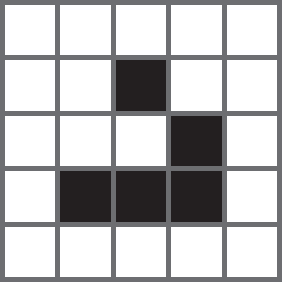
\includegraphics[width=\linewidth]{figures/glider.pdf}
    \caption{Moving oscillator\\ (\emph{glider}).}
    \label{fig:glider}
  \end{subfigure}
  \begin{subfigure}[t]{.31\linewidth}
    \centering
    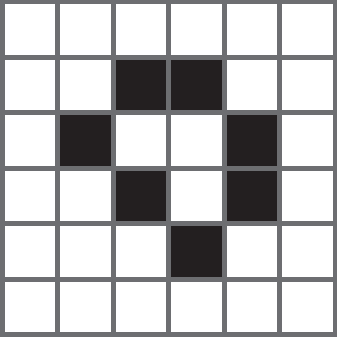
\includegraphics[width=\linewidth]{figures/still_life.pdf}
    \caption{Fixed pattern\\ (\emph{still life}).}
    \label{fig:still_life}
  \end{subfigure}
  \begin{subfigure}[t]{.31\linewidth}
    \centering
    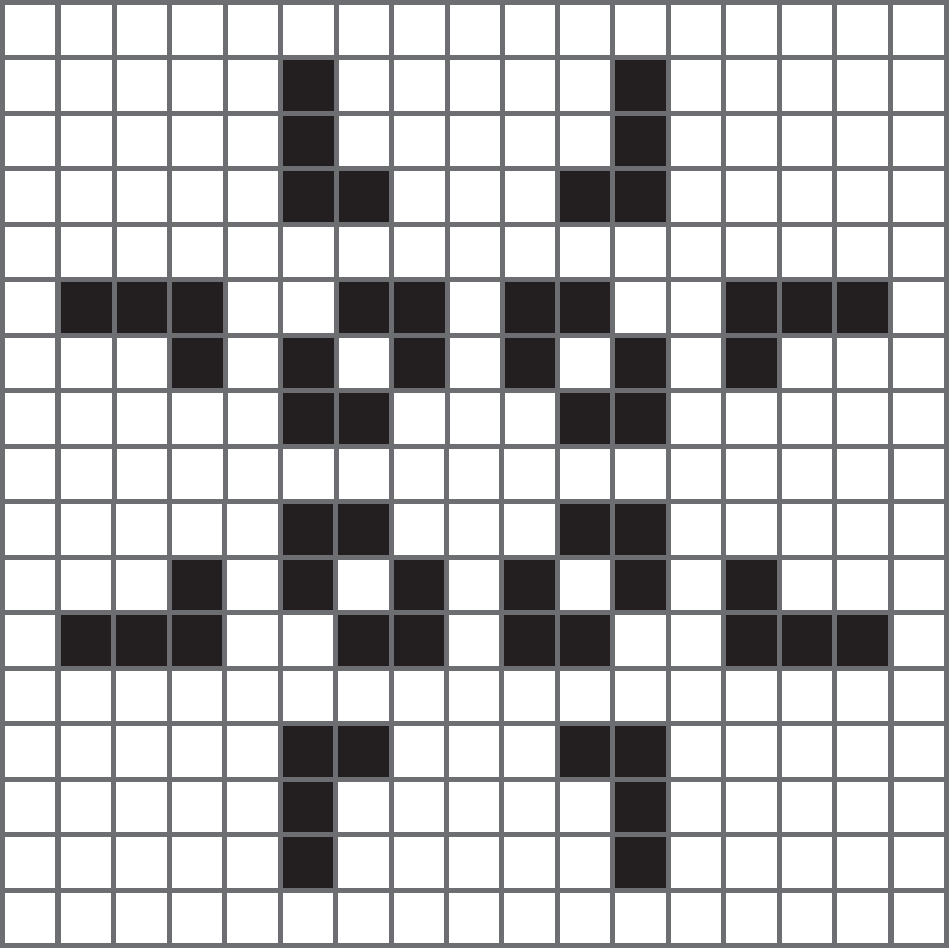
\includegraphics[width=\linewidth]{figures/pulsar.pdf}
    \caption{Period 3 oscillator\\ (\emph{pulsar}).}
    \label{fig:pulsar}
  \end{subfigure}

  \caption{Some game of life patterns with various properties. The moving
    oscillator \ref{fig:glider} moves 1 cell along the bottom right diagonal
    every 4 steps. The fixed pattern \ref{fig:still_life} never changes except
    if it interacts with others. The oscillator \ref{fig:pulsar} loops through
    three different configurations.}
  \label{fig:gol_patterns}
\end{figure}


\paragraph{Asynchronous cellular automata}
A cellular automaton is said to be asynchronous when its cells are not all
updated in parallel at each time step. Several cell update schemes can be
chosen. Contrary to regular cellular automata, the grid has to be finite for an
update rule to exist. This is because asynchronous \ac{CA} have to define an
order of update of the cells which would not be defined on an infinite grid.
This update order can be random, follow a predefined order, or be decided by a
global controller. Groups of cells can be updated simultaneously, or updates can
be done cell by cell. The many effects of the asynchronous updates can be hard
to predict and can make these types of \ac{CA} relatively hard to work with.

Asynchronous \ac{CA} are an appealing model when using large systems for which
parallel update is prohibitively expensive. The rule could adapt itself and
preferentially update cells in active or useful parts of the \ac{CA} while doing
slower updates to the less active parts of the \ac{CA}. An asynchronous \ac{CA}
with evolutionary properties was constructed in
\parencite{nehanivEvolutionAsynchronousCellular2003}. The authors argue that
asynchronicity is a strong advantage for constructing systems that can evolve
within \acp{CA}.

\paragraph{Stochastic cellular automata}
In a stochastic cellular automaton, the update function $\boldsymbol{\Phi}$ is
stochastic. This means that the next state of all cells in the grid is
sampled from a probability distribution that depends on the current neighborhood
configuration. We can write
\begin{equation}
\begin{aligned}
  \forall i \in \mathcal{L},\ s \in \mathcal{S} \quad p\left(c_{i}^{(t + 1)} = s \right) = \boldsymbol{\Phi} \left(\boldsymbol{N}\left(c_{i}^{(t)}\right)\right)(s).
\end{aligned}
\end{equation}
These \ac{CA} have had successful applications in physics
\parencite{vichniacSimulatingPhysicsCellular1984,
  ottaviSimulationIsingModel1989} or biology
\parencite{boasCellularPottsModel2018}, because their stochasticity allows
modeling complex physical phenomena.

\paragraph{Continuous}
Another family of \ac{CA} uses real-valued states, often restricted to the range
$[0, 1]$. The update function is then a real multivariate function, which we can
write
\begin{equation}
  \begin{aligned}
  \boldsymbol{\Phi}: [0, 1]^{s} \rightarrow [0, 1].
  \end{aligned}
  \label{eq:phi_cont}
\end{equation}

Examples of continuous \ac{CA} include Lenia which uses convolutional operators
followed by thresholding for the update rule
\parencite{chanLeniaBiologyArtificial2019a}, or \acp{NCA}
\parencite{mordvintsevGrowingNeuralCellular2020} which represents \acp{CA} as
neural networks (more details in Section \ref{sec:cell-autom-rnns} and
\ref{sec:neur-cell-autom}). \textcite{garzonRealComputationCellular1993}
explores the condition for a real-valued \ac{CA} to be able to compute
real-valued functions.

\paragraph{Higher dimensional cellular automata}
\acp{CA} of dimension higher than 2 have been comparatively less studied for
several reasons, including the limits that arise when simulating and visualizing
systems in more than 2 dimensions on a computer screen. Another problem is with
the increasing number of possible rules in higher dimensions. The number of
neighbors per cell grows exponentially with dimension, and the number of
possible rules has a doubly exponential rate of growth. This makes the
convenient representation of \acp{CA} rules as tables infeasible, since the size
of that table quickly exceeds the available memory of most computers. For
example, there are $2^{512} \approx 10^{154}$ possible 2D rules with 2 states and a
Moore neighborhood, which is already an incomprehensibly large number, but there
are $2^{134,217,728} \approx 10^{40,403,562}$ such rules in 3D.

Despite these limitations, several works have studied higher dimensions \acp{CA},
although mostly in 3 dimensions
\parencite{tsalidesThreedimensionalCellularAutomata1989,
  sudhakaranGrowing3DArtefacts2021}. For example, there are several examples of
successful 3D \acp{CA} simulations applied to material sciences
\parencite{gandin3DCellularAutomaton1997, arataFreeformShapeModeling1999,
  panStudyFailureScale2009, dicaprio3DCellularAutomata2016}.

\paragraph{Hexagonal cellular automata}
Hexagonal cellular automata are defined on grids tiled with hexagons, where each
cell has 6 direct neighbors.

\begin{figure}[htbp]
  \centering
  \begin{subfigure}[b]{.35\linewidth}
    \centering
    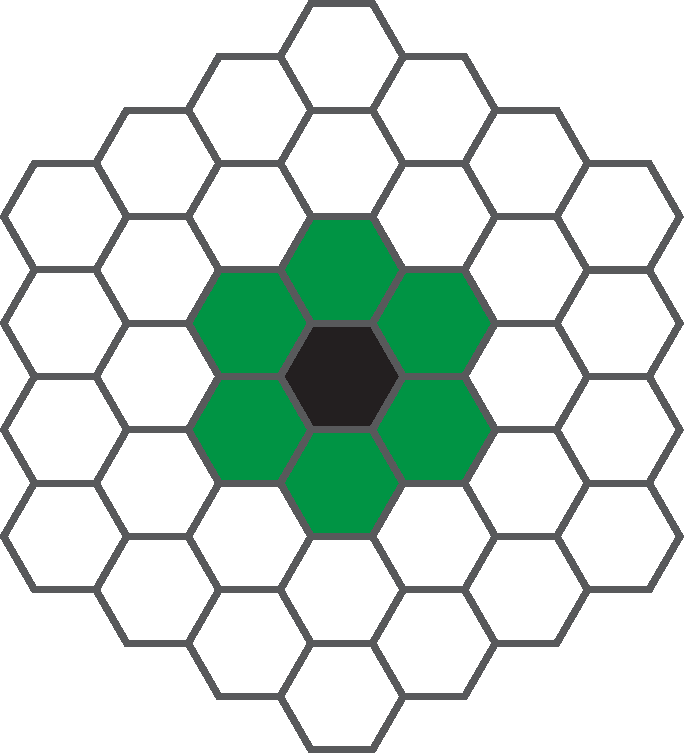
\includegraphics[width=\linewidth]{figures/hexagonal_1}
    \caption{Range 1 neighborhood}
    \label{fig:hexagonal_1}
  \end{subfigure}
  \hspace{10pt}
  \begin{subfigure}[b]{.35\linewidth}
    \centering
    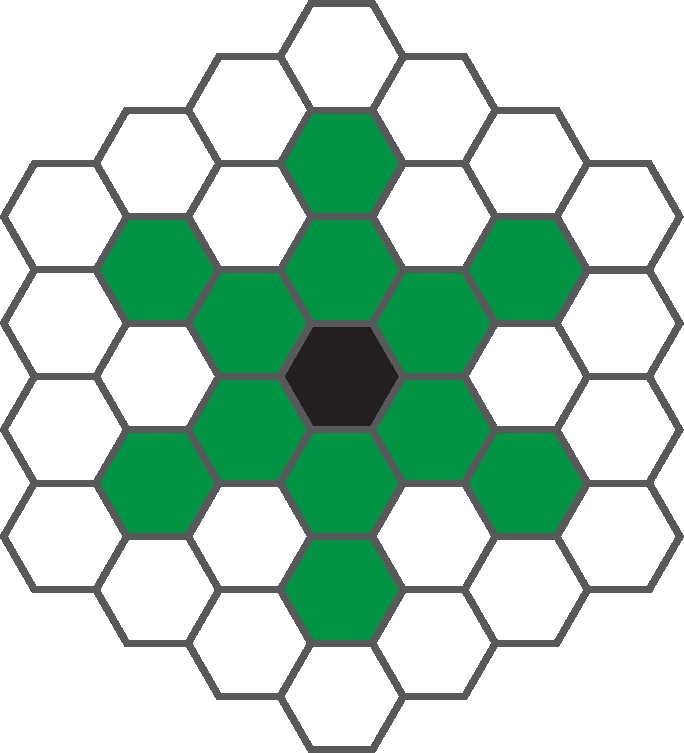
\includegraphics[width=\linewidth]{figures/hexagonal_2}
    \caption{Ray neighborhood}
    \label{fig:hexagonal_2}
  \end{subfigure}
  \caption{Example definition of neighborhood for hexagonal cellular automata.}
\label{fig:hexagonal}
\end{figure}

One advantage of this type of \acp{CA} over the regular grids is the absence of
preferred direction, since they are all equivalent. On a square grid, diagonally
adjacent cells span more distance that directly adjacent cells, whereas on an
hexagonal grid all neighbors are equivalent
\parencite{moreeHexagonalSquareLattice2004}.

\subsection{Parametrizing and sampling CA rules}
As explained in Section \ref{sec:challenges}, one of the main challenges of
working with complex systems is the parametrization and control of the behavior
of that system. \ac{CA} are no exception, and several parametrization schemes
have been proposed, having their respective benefits and drawbacks. There are
infinitely many ways to define rules for \acp{CA}, and for each of these
definition a very large number of rules is available, making it impossible to
sample a significant portion of the rule space. A good parametrization allows
scanning a wide range of behavior of \ac{CA} by traversing the space in an
interesting way.

\paragraph{Langton's lambda\label{sec:langtons-lambda}}

Christopher Langton proposed one of the first parameters that could be used to
control the behavior of \acp{CA} to a certain extent
\parencite{langtonStudyingArtificialLife1986, langtonComputationEdgeChaos1990}.
For a \ac{CA} with $K = |\mathcal{S}|$ states and a state arbitrarily chosen to
be the \emph{quiescent} state (this corresponds to the ``dead'' state in the
game of life, for example), if there are $n$ transitions to the quiescent state
within the rule table and $K^{s} - n$ remaining transitions that do not lead to
the quiescent state, where $s$ is the number of cells in the neighborhood, we
have

\begin{equation}
  \label{eq:langton}
  \begin{aligned}
    \lambda = \frac{K^{s} - n}{K^{n}}.
  \end{aligned}
\end{equation}

For Langton, the purpose of $\lambda$ is to search the space of \ac{CA} in an ordered
manner by varying the value of the parameter. His procedure starts with a rule
with all transitions leading to the quiescent state. The value of $\lambda$ is
increased in discrete steps to $1 - 1 / K^{n}$ by randomly changing the
transitions of the rule to lead to a different state. An illustration of the
behavior change of a \ac{CA} rule under this procedure is shown on figure
\ref{fig:langton_lambda}. Langton collected various measures of the dynamical
behavior of \ac{CA} and studied them as a function of $\lambda$. He observes a phase
transition as $\lambda$ approaches its maximal value, where the \acp{CA} seem to behave
in the most complex way, with long transients and large-scale propagating
structures. He calls this phase transition ``edge of chaos'' because it
corresponds to $\lambda$ values just before the generated \acp{CA} become
chaotic.

\begin{figure}[htbp]
  \centering
  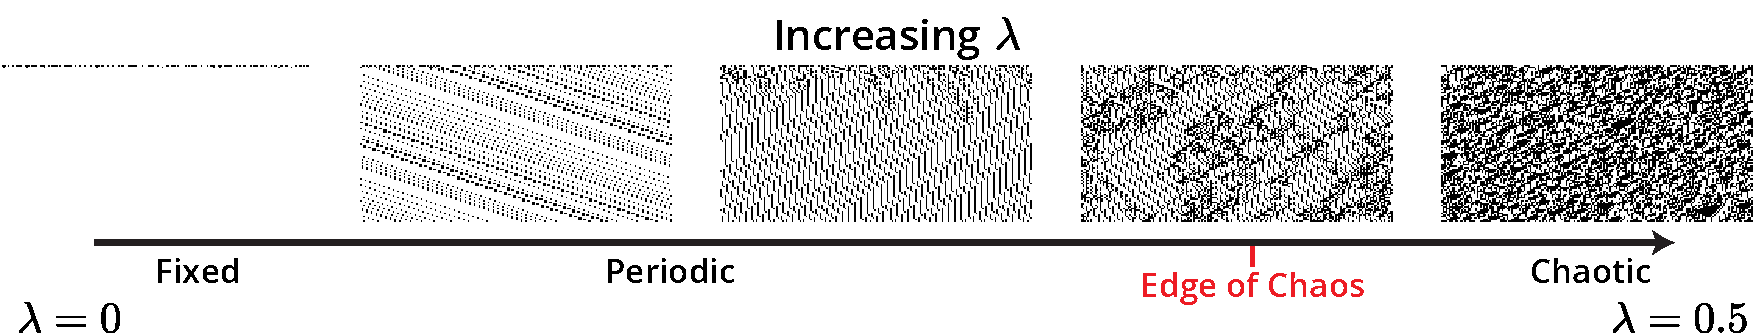
\includegraphics[width=\linewidth]{figures/langton_lambda.pdf}
  \caption{The effect of varying $\lambda$ for a 1D binary \ac{CA} rule. A \ac{CA}
    rule is progressively modified along a trajectory of increasing $\lambda$. The
    rule starts with a fixed behavior, becomes periodic and then complex when
    hitting the ``edge of chaos''. Note the localized structures that spread
    over time (down along the y axis) and interact in the fourth figure. When
    $\lambda$ increases further the rule becomes chaotic.}
  \label{fig:langton_lambda}
\end{figure}

\paragraph{Dirichlet sampling}
For an arbitrary number of states and arbitrary neighborhood size, it can be
challenging to sample \acp{CA} while scanning the wide range of behavior these
models are capable of simulating. This is because the size of the space of
\acp{CA} rules is very large. The naive method of uniformly sampling each
transition output is not useful in large rule spaces with multiple states, large
neighborhoods or grid dimension higher than 1.

Rules with equal proportions of transitions leading to all states tend to be the
most chaotic. This is also what Langton observed when studying the $\lambda$
parameter. This is explained by the fact that sampling each transition output
uniformly is equivalent to sampling the rules from a multinomial distribution
with the number of possible states ($K$), number of possible transitions
($n = K^{K^{s}}$, with $s$ the number of cells in a neighborhood), and uniform
probabilities $p_{1}= \ldots= p_{K}$ as parameters. A random variable
$X = (X_{1}, \ldots, X_{K})$ indicates the number of times each result is observed.
The probability mass function of this distribution is

\begin{equation}
  \label{eq:multinomial}
  \begin{aligned}
    P(X_{1}=x_{1}, \ldots , X_{K}=x_{k}) = \frac{n!}{x_{1}!\cdots x_{K}!} p_{1}^{x_{1}}\cdots p_{K}^{x_{K}}.
  \end{aligned}
\end{equation}

This quantity becomes vanishingly small for large $n$ (that is rules with many
states or large neighborhoods) and rules with an output transition skewed
towards a specific state. For example, the binary game of life rule has 372
transitions that lead to state 0 and 140 that lead to state 1. The probability
of sampling a rule with these transition proportions is $8.24\mathrm{e}{-26}$
(compared to a $17\%$ chance of sampling a rule with between 254 and 257
transition to 0). It is therefore very unlikely that a rule of the type of game
of life, let alone the rule itself, would be obtained with a uniform transition
sampling method.

We propose a Dirichlet sampling method as an alternative way to sample rules
with fixed ratios of transitions leading to each output states. For a rule with
$K$ states, we sample a $K$-uple from a Dirichlet distribution of order $K$ with
parameters $(\alpha_{k})_{k\in [1, K]}$ where $\alpha_{0} = \alpha_{1} = \ldots = \alpha_{K} = \alpha < 1$. The
result is a quantile $K$-uple $(q_{1}, \ldots, q_{K})$. For $\alpha < 1$, the distribution
is concentrated around the corners of a simplex of dimension $K$, which means
that it preferably samples tuple with one of their values dominating the others.

Rules are sampled so that the number of transition to each output state matches
the quantile generated from the Dirichlet distribution. Samples will be more
likely to have a dominant quantile which can be associated with the quiescent
state in Langton's $\lambda$ calculation. The resulting sampling of cellular automata
is much better for scanning the whole space of rules and generating \ac{CA}
rules which would be unreachable with the naive sampling method, as illustrated
on figure \ref{fig:ca_rule_sampling}.

\begin{figure}[htbp]
  \centering
  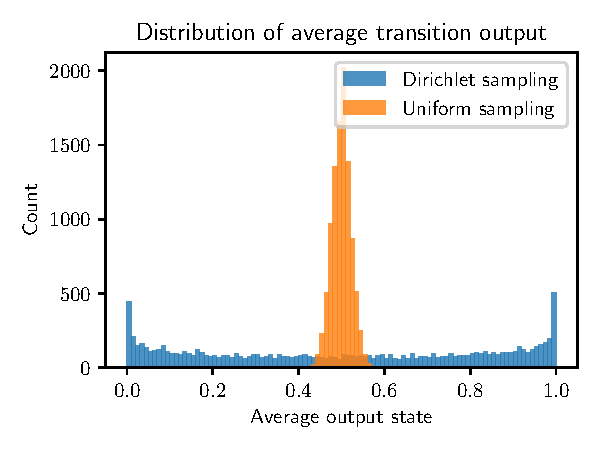
\includegraphics[width=.5\linewidth]{figures/ca_rule_sampling_hist}
  \caption{An illustration of the difference between naive uniform rule sampling
    and Dirichlet sampling on binary rules. 10000 2D binary CA rules were
    sampled with each method, the plot displays an histogram of their average
    output state. Uniform sampling leads to more rules with an average output
    state close to 0.5, meaning approximately as many transitions towards both
    states. Dirichlet sampling can control, through the choice of parameter $\alpha$,
    how much rules with more skewed transitions should be sampled which is
    visible with the spiked on the blue histogram close to 0 and 1.}
  \label{fig:ca_rule_sampling}
\end{figure}

\paragraph{Smooth sampling with the recurrent convolutional neural network
  analogy.}

The recurrent convolutional network analogy of \acp{CA} (see Section
\ref{sec:cell-autom-rnns} for details) formulates a \ac{CA} as a neural network.
In this paradigm, the rule of a \ac{CA} is entirely determined by the parameters
of that neural network. This allows modifying the \ac{CA} rules like we would
change the weights of a neural network. For example, as long as all simulation
steps are differentiable, the backpropagation algorithm can be applied and used
to update a \ac{CA} rule by updating the weights of the neural network with
gradient descent. Dimensionality reduction methods applied to the parameter
space of the neural network can help understand the structure of that space and
the \acp{CA} behaviors that different sets of parameters produce.


\section{Cellular automata and RNNs}\label{sec:cell-autom-rnns}

The purpose of this section is to show that cellular automata and recurrent
convolutional neural networks have very strong connections and to draw this
parallel as clearly as possible. We express the \ac{CA} update function as a set
of convolutional operations that can be derived from any \ac{CA} rule.

This connection yields interesting consequences both for the theoretical
properties of these models and the potential applications of \acp{CA} and
recurrent networks. It shows for instance that emergent properties with
increasing complexity and perhaps open-ended development that we expect from
complex systems such as \acp{CA} are possible within the hidden state of a
recurrent neural network.

The conceptual similarity between \acp{CA} and neural networks is not surprising. 
Fundamentally, \ac{CA} represent the paradigm of emergence, in which
the origins of complex behaviors are searched for in an assemblage of possibly
very simple parts rather than being viewed as a sum of complex building blocks. It is
often argued that there is no better known example of a truly emergent
phenomenon than that of the emergence of consciousness out of the large network
of functionally simple (and certainly unconscious) neuronal components that make
up the human brain. A biological neural network, such as a \ac{CA}, consists of a
large space of interconnected nodes, with a dynamical behavior that is a local
function of the other nodes to which it is connected. Artificial neural networks can
be thought of as being a set of biologically inspired CA rules
\parencite{ilachinskiCellularAutomataDiscrete2001}. The more precise parallel
between cellular automata and a form of recurrent/convolutional network has also
been drawn by several other researchers
\parencite{wulffLearningCellularAutomaton1993,
  gilpinCellularAutomataConvolutional2018,
  mordvintsevGrowingNeuralCellular2020}.

In this section we formally describe the relation between \acp{CA} and \acp{RNN}
and discuss the extensions this implies for the \ac{CA} model as well as some of
the consequences of that relation.

\subsection{RNN formalism}

\begin{figure}[htbp]
  \centering
  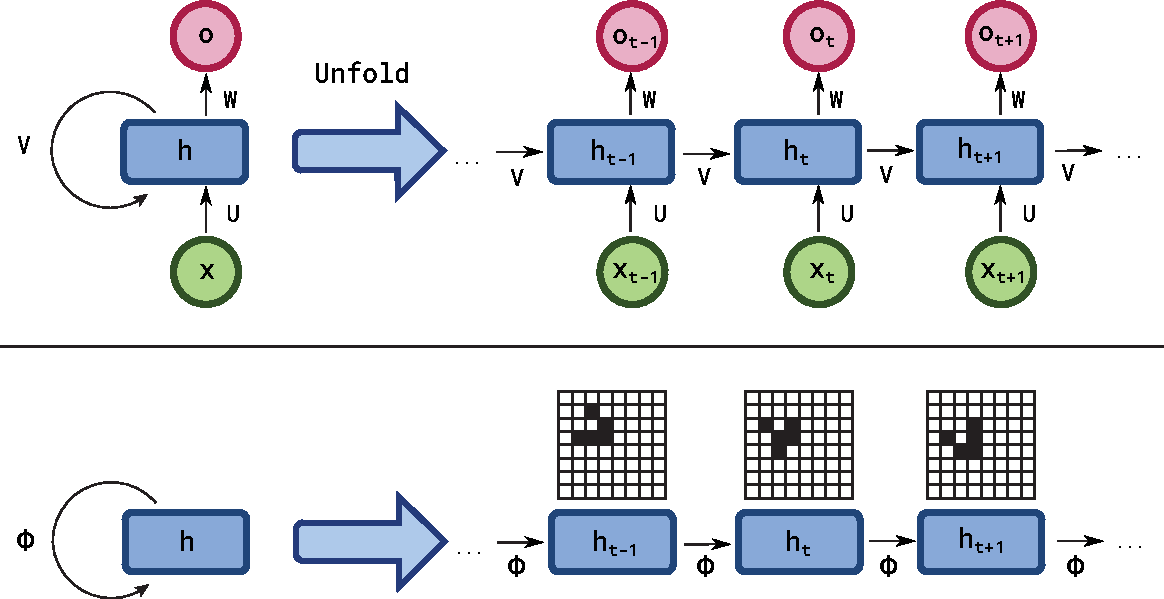
\includegraphics[width=\linewidth]{figures/rnn_and_gol.pdf}
  \caption{\label{fig:standard_rnn} Standard RNN architecture (left) and Game of
    Life seen as a RNN with no inputs and outputs (right). For the \ac{CA}, the
    ``hidden'' state $h_t$ is the current state of the grid at timestep $t$. The
    operator $\boldsymbol{\Phi}$ is the \ac{CA} update rule which is
    equivalent to a \ac{CNN} (see Section~\ref{sec:transition-rule-as}). This
    illustration is based on
    \href{https://commons.wikimedia.org/wiki/File:Recurrent_neural_network_unfold.svg}{Recurrent
      neural network unfold} by
    \href{https://commons.wikimedia.org/wiki/User:Ixnay}{fdeloche}, licensed
    under \href{https://creativecommons.org/licenses/by-sa/4.0/}{CC BY 4.0}.}
\end{figure}


\begin{figure}[htbp]
  \centering
  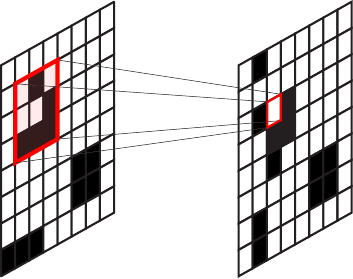
\includegraphics[width=.3\linewidth]{figures/ca_cnn}
  \caption{\label{fig:ca_cnn}The CA update rule is local and can be represented
    by a convolutional neural networks: linear local uniform transformations
    followed by the application of a non-linear function.}
\end{figure}

We write the definition of a \ac{CA} with \ac{RNN}-inspired formalism and
notation. This parallel is illustrated in figures \ref{fig:ca_cnn} and
\ref{fig:standard_rnn}. The grid state at time $t$ is denoted $h_t$ and
corresponds to the hidden state in a RNN\@. In the case of classical \acp{CA},
it is a 1 or 2D vector of discrete values (see Section \ref{sec:definition}),
but~\parencite{mordvintsevGrowingNeuralCellular2020} and other \acp{CA}
extensions use continuous values, much like the usual \acp{RNN}.

The transformation $\Phi$ operates only on the hidden state. Because it is local,
it can be shown to be equivalent to a convolutional layer, as explained below in
Section~\ref{sec:transition-rule-as}. Inputs and outputs
$(\mathbf{x}, \mathbf{o})$ from figure \ref{fig:standard_rnn} are not included
in the classical definition of CAs but are an easy to implement extension as
discussed in Section~\ref{sec:adding-inputs-outp}.

\subsection{Transition rule as a set of convolutions\label{sec:transition-rule-as}}

Each cell $c_i$ from the \ac{CA} definition can be in one of $k$ states. We
represent the cells as vectors of size $k$ the number of states, with only
zeroes expect for a one in the $k$-th position. A neighborhood of size $3$ in a
1D CA can be represented as a $3 \times k$ vector
$\mathbf{u}_i = [u_{i-1}, u_{i}, u_{i+1}]$. Each $u_{i}$ is a vector of size $k$
with a $1$ in position $s_i$. This is illustrated in the 1D (resp.\ 2D) case on
the left (resp.\ right) of Figure~\ref{fig:cell}. For a CA with only two states,
it is redundant to have a $3 \times 2$ vector, but the ``one-hot'' encoding
becomes useful when working with more states.

\begin{figure}[htbp]
  \centering
  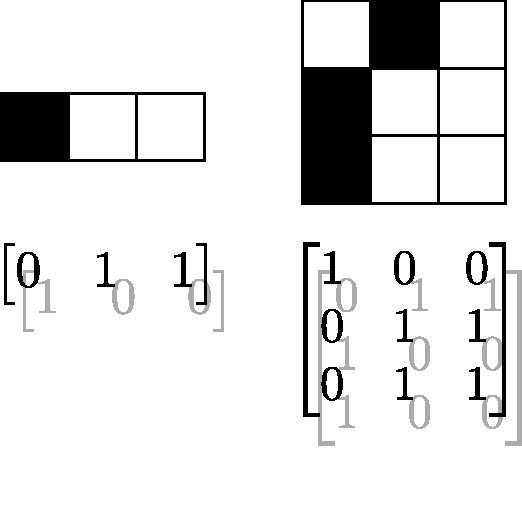
\includegraphics[width=.4\linewidth]{figures/repr}
  \caption{\label{fig:cell}A \ac{CA} neighborhood vector representation example
    with 2 states. A $3\times 3$ square of cells with two states can be represented
    by a $3\times 3 \times 2$ vector. Left: 1D 3-neighbors representation. Right: 2D $3\times3$
    neighbors representation. The last dimension of the vector encodes a
    ``one-hot'' representation of the state of the cell.}

\end{figure}

With this representation, we can express the transition rule $\Phi$ as a simple
convolutional neural network. This network would be made up of 2 layers, which
are shown in Figure~\ref{fig:ca_cnn_2dims} for the 2D case:

\begin{figure}[htbp]
  \centering
  \begin{subfigure}[b]{\linewidth}
    \centering
  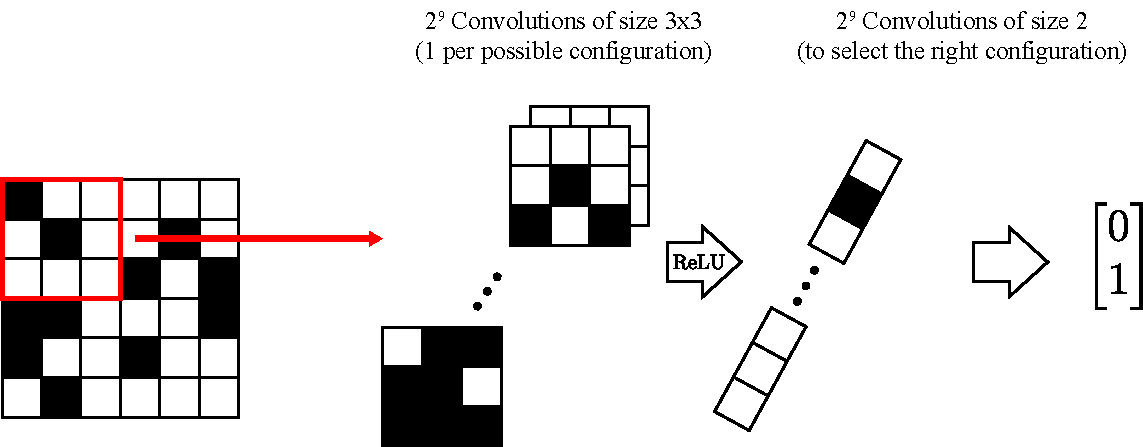
\includegraphics[width=.9\linewidth]{figures/global_schema}
  \caption{\label{fig:global_schema}A representation of any 2-states 2D CA rule
    operating on $3\times 3$ neighborhoods as a 2 layers CNN. There are 512 filters
    receptive to each $3\times 3$ neighborhood states in the first layer. The second
    layer determines the output value for each neighborhood state.}
  \end{subfigure}
  \begin{subfigure}[b]{\linewidth}
    \centering
  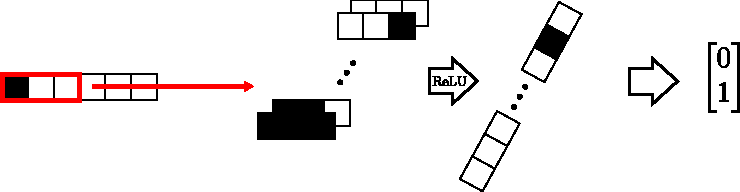
\includegraphics[width=.9\linewidth]{figures/one_d_global_schema}
  \caption{\label{fig:one_d_global_schema}A representation of any 2-states 1D CA
    rule operating on neighborhoods of size 3 as a 2 layers CNN. There are 8
    filters of size 3 in the first convolutional layer, and 8 filters of size 1
    in the second one.}
  \end{subfigure}
  \caption{Two examples of \acp{CA} rules represented as a simple CNN. Padding
    ensures the grid obtained after the CNN step is of the same size as the
    original grid.}\label{fig:ca_cnn_2dims}
\end{figure}


\paragraph{The first convolutional layer.} It is receptive to each possible
neighborhood configuration. In the 1D case with neighborhood size 3, this is all
eight configurations $000, 001, 010, \ldots, 111$. For a radius $r$ in 1D, this layer
is composed of $k^{2r + 1}$ filters of dimension $k \times (2r + 1)$ with only ones
and zeros, which are the mirror of a possible configuration of size $(2r+1)$ of
the neighborhood.

The product of each filter with an input neighborhood on the grid will be an
integer between $0$ and $2r + 1$. By applying a ReLU nonlinearity preceded by a
constant vector of value $2r$ as bias, we obtain the input to the second layer,
a vector of size $k^{2r + 1}$ for each cell containing all zeroes except for a
one corresponding to the detected neighborhood. This vector plays the role of an
indicator of the current input configuration.

\paragraph{A second convolutional layer} It has $k^{2r + 1}$ filters of size $1$
that are $0$s or $1$s depending on the desired output value of that transition.
When applied on the indicator vector above, the obtained output will be the
output value of the rule corresponding to the detected neighborhood state.

With some circular padding that wraps around the edges of the grid or applies
constant values outside of the main grid, the size of the output is the same as
the input. This means the CNN step can be applied multiple times, simulating a
single \ac{CA} step every time.

\subsubsection{Recurrent convolutions in machine learning}

Recurrent convolutional networks have been used in some areas of machine
learning such as NLP or computer vision
\parencite{pinheiroRecurrentConvolutionalNeural2014,
  laiRecurrentConvolutionalNeural2015}.

\subsection{Adding inputs and outputs\label{sec:adding-inputs-outp}}

Figure~\ref{fig:standard_rnn} shows clearly where the inputs and outputs could
be added to the Game of Life or any other \ac{CA}. We list many possible forms
the input and outputs can take, and how it can interact with the \ac{CA} rule.

\subsubsection{Inputs}
There are many ways to add inputs to the recurrent \ac{CNN} model presented
above. We divide our proposed methods into two classes: inputs that directly
modify the hidden state during the CA evolution and inputs that augment the
hidden state without changing it directly and affect the rule.


\paragraph{Hidden-state augmentation and rule modulation.}
Inputs are usually added to the hidden state just before the application of the
nonlinearity in standard RNNs.

In the case of cellular automata, it can also be done in the following ways:

\begin{figure*}[ht]
  \centering
  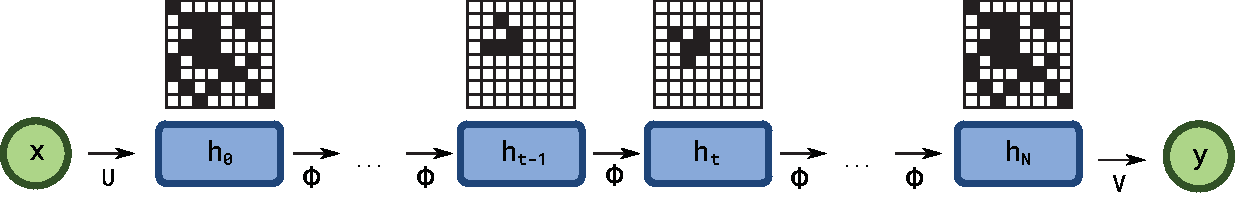
\includegraphics[width=.9\linewidth]{figures/encode_decode.pdf}
  \caption{\label{fig:encode_decode} Inputs and outputs can be directly
    encoded within the hidden state.}
\end{figure*}

\begin{itemize}
  \item \textbf{Vector state.} A naive way to add inputs to a \ac{CA} is to
        consider the grid as having an additional (possibly read-only)
        dimension. For example, a 1D automaton would actually be represented by
        a vector of dimension $N\times 2$ where the first vector of size $N$ is the
        state of the grid and the other is the input. The update rule would be
        changed to add this new component into account. One can see this model
        as using multiple CA rules at the same time, with the input state
        conditioning the rule being chosen for a given update step.

  \item \textbf{Variable update rule.} Inputs can also influence a CA's evolution by
        changing the update rule. With this configuration, the update rule $\Phi$
        is now a function of the input $x$. We now have $\Phi_x = G(x)$, where

        \[G: \mathcal{X} \rightarrow \left({\{ 1, \ldots, k \}}^{2r+1} \to \{1, \ldots, k\}\right)\]


        A similar approach was used in
        \parencite{adamsFormalDefinitionsUnbounded2017}. It showed that
        conditioning a CA update rule on another CA's evolution could enable a
        higher diversity of behavior.

  \item \textbf{Concatenation.} Input can be concatenated to the hidden state (\eg~on
        the grid boundaries) before applying the update rule, forming a sort of
        fixed read-only memory space. The concatenation is illustrated in
        Figure~\ref{fig:concat}. A possible disadvantage of this method is the
        fact that information needs to propagate through the grid if it is to be
        processed far from where the read-only memory was positioned.

        This approach is more computer-like, reserving some space for different
        functionalities of the data.

\begin{figure}[ht]
  \centering 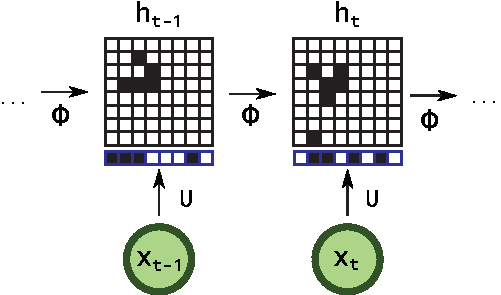
\includegraphics[width=.5\linewidth]{figures/concat.pdf}
  \caption{\label{fig:concat} Input $x_t$ is projected and concatenated to
    hidden state $h_t$, affecting the boundary conditions of the 
    \ac{CA}. For the \ac{CA}, this vector is just like another part of the
    hidden state except that it is not writable}
\end{figure}
\end{itemize}


\paragraph{Hidden-state manipulation.}
Another approach is to directly modify the hidden state to ``communicate''
information to the system. These methods are used
in~\parencite{mordvintsevGrowingNeuralCellular2020,
  randazzoSelfclassifyingMNISTDigits2020} to make interactive demos and allow
users to directly modify that hidden state. A user can interact with the system
by drawing with its mouse. This sets parts of the internal state to a fixed cell
state.

\begin{itemize}
  \item \textbf{Masking.} Input data can serve as a mask on top of the current
        grid state, forcing some cells into states that depend on the input
        values. If we view the state activations in the CA as some neural
        pattern, this approch can be seen as a form of \emph{neuromodulation},
        which has previously been used in machine learning
        \parencite{soltoggioEvolutionaryAdvantagesNeuromodulated2008,
        ishiguroNeuromodulatedControlBipedal2003,
        beaulieuLearningContinuallyLearn2020}.

        A mask can be constructed from an input vector $x$ by linearly
        transforming $x$ and applying an activation function (\eg~step
        function). It controls which channels are activated, and where
        information can flow or not. This kind of mask can be applied with
        element-wise multiplication or addition but also more elaborate
        operations. It is illustrated in Figure~\ref{fig:mask}.

\begin{figure}[ht]
  \centering
  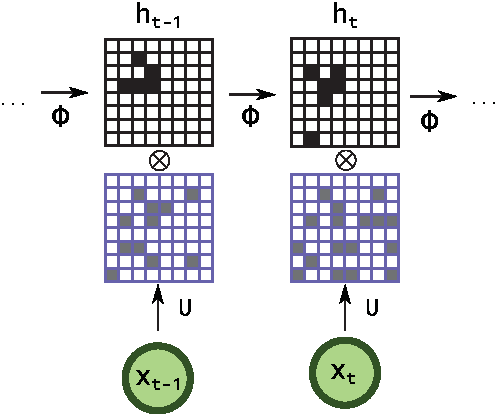
\includegraphics[width=.5\linewidth]{figures/mask.pdf}
  \caption{\label{fig:mask} Input is converted into a binary mask for the hidden
    state. The mask is applied through element-wise multiplication here.}
\end{figure}

\end{itemize}

\subsubsection{Outputs}

Similarly, inputs can be extracted from the hidden state in several different
ways. One might read outputs from the boundaries of the grid, from a
transformation of the grid using a neural network, etc. The output could also be
stored within an additional dimension of the ``extended'' grid state presented
above.

\subsubsection{Cellular automata and computations}

From a computational point of view, the hidden state can be seen as a working
tape that some kind of \emph{parallel Turing machine} (the cellular automaton)
is performing computations on. In this framework, the input is encoded as the
initial state of the tape and decoded from the last state of the tape (as
illustrated on Figure~\ref{fig:encode_decode}). The recurrent convolutional
neural network (RCNN), or \ac{CA}, then plays the role of a fixed computer
program which is executed. This is the setting adopted in previous works on
constructing computations with cellular automata: a task is chosen, and one
searches for rules which can execute that task on input/output
pairs~\parencite{mitchellComputationCellularAutomata2005}. Previous successes
with \acp{RNN} demonstrate that this model is powerful enough to learn complex
functions when the grid is made of continuous numbers and the transformation is
not local thanks to optimization, for instance in language modeling.

However, another interesting point of view can be taken when we consider the
hidden state (or tape) as encoding both some data and a computer program, as is
the case with a Turing machine. We can then expect a \ac{CA} (or \ac{RNN}) not
only to compute the result of a particular function but to be equivalent to a
general-purpose computer capable of computing the result of any chosen algorithm
without any need for optimization. Making a universal \ac{CA} compute some
program amounts to encoding the program into the right language and
communicating it by embedding it within the hidden state. In practice, figuring
out the right encoding is often the biggest challenge. This is also the reason
that the few Turing complete \ac{CA} are not so useful in practice, since we do
not know of any efficient encoding for programming them.

\subsection{Consequences}

Viewing cellular automata as recurrent convolutional neural networks, like
described above has several interesting consequences, of which we list a few
here.

\subsubsection{Turing-completeness of the system}

Because we can simulate rule 110 ECA in the above RCNN system, it follows from
the Turing completeness of this CA rule that the RCNN is Turing complete. This
is an interesting result, although not very significant since \acp{RNN} have
already been proven to be Turing
complete~\parencite{siegelmannComputationalPowerNeural1992}, with very little
practical implications. Our model is relatively far from a real-world CNN with a
fixed number of layers independent from one another --- compared to a variable
number of steps and shared layers for the automaton-RCNN. Thus this property
does not bear any consequence on \acp{CNN}.

\subsubsection{Differentiable cellular automata}

Every step of the computations involved in computing a step of a cellular
automaton represented as a RCNN is differentiable. Therefore, we can
theoretically couple this framework with backpropagation to create
\emph{learnable} cellular automata that can adapt their rules to minimize a
target loss function.

This is the direction taken by~\textcite{mordvintsevGrowingNeuralCellular2020}.
The authors use supervised learning on a cellular automaton and train it to get
a stable self-repairing target shape. However, because supervised cellular
automata can only do as much as they have been trained to do, it may defeat the
purpose of working with a model capable of spontaneous complex emergent
behavior. An open-ended complexity increase could very unlikely be achieved
through pure supervision.

\textcite{gilpinCellularAutomataConvolutional2018} takes the reverse approach
and tries to train RCNNs to simulate a fixed CA rule, using the statistics of
that training process as a way to help understand the structure of CA rule
space.

\subsection{Beyond the naive rule representation}

The above representation of cellular automata rules is a one-to-one mapping.
Each automata rule has its CNN counterpart and vice versa. However, there are
more efficient ways to represent CA rules. For instance, we can make the first
layer of filters receptive both to a given configuration and its inverse
(\eg~$(1, 0, 1)$ and $(0, 1, 0)$ in a ECA) by using negative values in the
filter (use a filter $(1, -1, 1)$ instead of $(1, 0, 1)$ and $(0, 1, 0)$
separately).

For example, game of life does not need more than 2 convolutional filters or
parameters to be represented by a CNN because it is totalistic (a cell's new
state only depends on the number of neighbors in state 1 and its current state).


\section{Reservoir computing \label{sec:res-models}}
\Ac{RC} is a computational framework that aims to exploit the states of a
complex dynamical system to perform some target task
\parencite{tanakaRecentAdvancesPhysical2019}. It relies on a \emph{reservoir} of
computations, that is, a dynamical system performing operations on its internal
state. An input signal is fed into this reservoir that behaves as a black box
from the point of view of the algorithm. Input values can be sequential or
nonsequential. They are projected and combined with the dynamical system using
a suitable mechanism. This projection can be learned, set randomly, or chosen.
The internal state of the dynamical system evolves according to its update
rule. Finally, the a decoder model (usually a linear regression) is trained in a
supervised manner to extract necessary information from the internal state of
the dynamical systems to predict the right output. A general diagram describing
this process is shown in figure \ref{fig:reservoir_diagram}.

\begin{figure}[htbp]
  \centering
  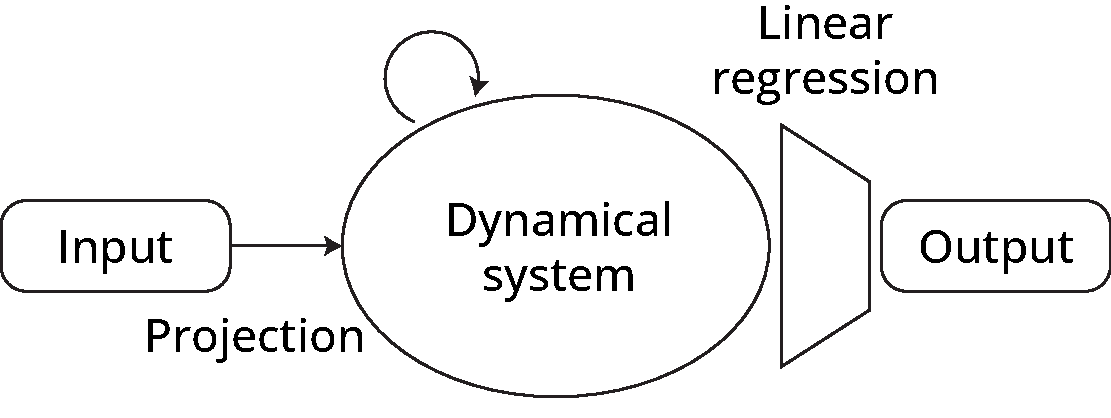
\includegraphics[width=.8\linewidth]{figures/reservoir_schema}
  \caption{Diagram of the general functioning of a \ac{RC} system. Input values
    are projected in the state or evolution function of a dynamical system which
    is run according to its internal rule. Output values are decoded from the
    internal state of the dynamical systems with a trainable layer.}
  \label{fig:reservoir_diagram}
\end{figure}

Some early known formulations of \ac{RC} are due to
\textcite{kirbyContextDynamicsNeural1991}. Another early formulation of the idea
was done by \textcite{schomakerNeuralNetworkModels1990,
  schomakerSimulationRecognitionHandwriting1991,
  schomakerNeuralOscillatornetworkModel1992}.

In another early work, \textcite{buonomanoTemporalInformationTransformed1995}
used a random spiking neural network with excitatory and inhibitory elements.
Neuron connection probabilities were inspired by real rat brain data
\parencite{masonSynapticTransmissionIndividual1991}. He observed a interval
sensitive response of these neurons when subjected to pulses spaced by varying
time intervals. This indicates an ability to encode temporal information. To
measure this phenomenon he trained an output linear layer to recognize specific
patterns in the activation of the last layer of neurons. This idea of using a
randomly initialized neural network with fixed weights and train a simple linear
layer to decode outputs was reinvented later under the names ``Echo-state
networks'' \parencite{jaegerEchoStateApproach2001} and ``Liquid state machines''
\parencite{maassRealTimeComputingStable2002}.

Another advantage of reservoir computing is that the reservoir can be
implemented using a variety of physical systems, substrates, and devices. These
types of reservoir are sometimes called ``exotic''
\parencite{lukoseviciusReservoirComputingApproaches2009}, but physical \ac{RC}
shows promise to develop cheap and efficient machine learning hardware and can
inform us on the nature and behavior of the underlying physical systems.
\textcite{tanakaRecentAdvancesPhysical2019} identifies four characteristics that
make a reservoir suitable for solving a computational task:

\begin{enumerate}
  \item The inputs need to be mapped to a high-dimensional space, which
        corresponds to the internal state of the reservoir. This
        high-dimensionality ensures that the inputs are separated with high
        probability.

  \item The reservoir should be non-linear. This will allow inputs that are not
        linearly separable to be separated as they are projected within the
        reservoir.

  \item The reservoir should have the echo-state property
        \parencite{jaegerEchoStateApproach2001, yildizRevisitingEchoState2012},
        or fading memory \parencite{boydFadingMemoryProblem1985,
        maassRealTimeComputingStable2002, maassFadingMemoryKernel2004}. This
        property relates asymptotic properties of the excited reservoir dynamics
        to the driving signal. A reservoir with the echo-state property will
        asymptotically forget all input values. This make some reservoir unable
        to solve tasks where unbounded memory is possibly required, such as
        context-free grammar parsing
        \parencite{schmidhuberTrainingRecurrentNetworks2007}. Later, reservoir
        models that address this issue were developed
        \parencite{pascanuNeurodynamicalModelWorking2011}.

  \item A reservoir should separate responses from different signals into
        different parts of the space, while being insensitive to small
        perturbations of the input. For a given system, this trade-off is often
        obtained at the transition between chaotic and non-chaotic regimes
        \parencite{bertschingerRealtimeComputationEdge2004,
        legensteinEdgeChaosPrediction2007}.
\end{enumerate}

We list common types of \ac{RC} below:

\begin{description}
  \item[Dynamical systems] The \ac{RC} models based on other reservoirs than
        random \acp{RNN}. This includes reservoir computing with \aclp{CA},
        which we give more detail about in section \ref{sec:app-ca-res}.
  \item[Electronic \ac{RC}] These models are implemented on electronic circuits,
        such as artificial neural networks implemented on physical circuits or
        other neuromorphic circuits. For example, \ac{RC} models can be build on
        FPGAs \parencite{antonikApplicationFPGAReal2018,
        verstraetenReservoirComputingStochastic2005,
        alomarLowcostHardwareImplementation2014,
        antonikFPGAImplementationReservoir2015} or memristive circuits
        \parencite{yangInvestigationsStaircaseMemristor2016,
        merkelMemristiveReservoirComputing2014,
        donahueDesignAnalysisNeuromemristive2015}.
  \item[Mechanical \ac{RC}] Soft mechanical bodies have complex nonlinear
        dynamics that can be beneficial to build a \ac{RC} model
        \parencite{pfeiferHowBodyShapes2007}. For example, a reservoir using a
        mass-spring network was proposed by
        \textcite{hauserTheoreticalFoundationMorphological2011}.
  \item[Biological \ac{RC}] There have been multiple hypotheses on whether the
        parts of the brain behave like a \ac{RC} system
        \parencite{yamazakiCerebellumLiquidState2007}. For example, a \ac{RC}
        model was proposed to understand the mechanism of context-dependent eye
        movement \parencite{domineyComplexSensorymotorSequence1995,
        domineyModelCorticostriatalPlasticity1995}.
  \item[Photonic \ac{RC}] The principle of photonic \ac{RC} is to use optical
        reservoirs to generate the computations. A first example using
        semiconductor optical amplifiers (SOAs) was proposed by
        Vandoorne and colleague \parencite{vandoorneOpticalSignalProcessing2008,
        vandoorneParallelReservoirComputing2011} and subsequently built \parencite{vandoorneExperimentalDemonstrationReservoir2014}.
        The photonic implementation of reservoir computing is based on the idea that
        photonic accelerators \parencite{kitayamaNovelFrontierPhotonics2019} can
        realize fast information processing with low
        learning costs \parencite{paquotOptoelectronicReservoirComputing2012,
        martinenghiPhotonicNonlinearTransient2012,
        suganoReservoirComputingUsing2020, antonikHumanActionRecognition2019}.
        Some of the implementations use the scattering of light in complex media
        \parencite{dongOpticalReservoirComputing2020,
        rafayelyanLargeScaleOpticalReservoir2020}.
  \item[Spintronics \ac{RC}] Some \ac{RC} works used nanosacle electronics
        involving the charge and spin of electrons called \emph{spintronics}
        \parencite{wolfSpintronicsSpinBasedElectronics2001}. Spintronics have
        been used in multiple ways to build \ac{RC} models, using spin torque
        oscillators (STO)
        \parencite{torrejonNeuromorphicComputingNanoscale2017,
        williameChaoticDynamicsMacrospin2019}, or spin waves
        \parencite{nakaneReservoirComputingSpin2018}.
\end{description}

\subsection{Reservoir computing applications}

\ac{RC} has had successful applications in various fields. It has been applied
for pattern classification; in audio with spoken digit recognition
\parencite{verstraetenIsolatedWordRecognition2005} and waveform classification
\parencite{paquotOptoelectronicReservoirComputing2012}; in computer vision with
written digits recognition \parencite{jalalvandRealTimeReservoirComputing2015},
and human motion classification \parencite{sohIterativeTemporalLearning2012,
  antonikHumanActionRecognition2019}. Another popular application of \ac{RC} is
time-series forecasting \parencite{jaegerEchoStateApproach2001,
  jaegerAdaptiveNonlinearSystem2002, wyffelsComparativeStudyReservoir2010}.
\ac{RC} has also been used in reinforcement learning to control agents in
artificial environments \parencite{kannoPhotonicReinforcementLearning2022} or
learn radio spectrum access \parencite{changDistributiveDynamicSpectrum2019}.

\subsection{Echo-state network}

The \acf{ESN} (and simultaneously developed model \emph{Liquid state machine}
(LSM)) is the most well-known implementation of the \ac{RC} principle
\parencite{tanakaRecentAdvancesPhysical2019}. The main idea behind this model is
to drive a \ac{RNN} with some input signal, which will excite the neurons within
the reservoir and induce several nonlinear response signals. This is combined
with a trainable linear regression to extract a desired output from a
combination of these response signals.

In practice, the input projection is often fixed but it can also be trainable.
The output can also be fed back to the reservoir like an input, and the
structure of the \ac{RNN} reservoir can be adapted.

\begin{figure}[htbp]
  \centering
  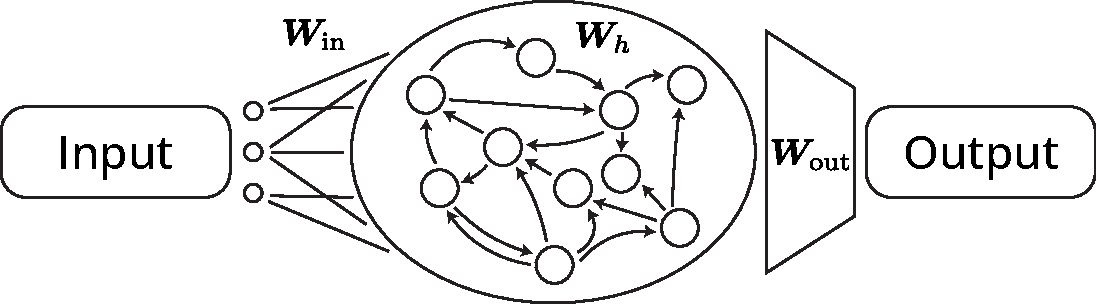
\includegraphics[width=.8\linewidth]{figures/echo_state_network}
  \caption{Diagram of an echo-state network. The \ac{RNN} is reprensented
    ``flattened'' in time. The circles represent the units of the hidden state
    of the \ac{RNN}. An arrow between unit $i$ and $j$ corresponds to a non-zero
    entry in the matrix, $\mW_{h, ij} \neq 0$. Non-linear operations are not
    represented.}
  \label{fig:echo_state_network}
\end{figure}

We define an input sequence to be $(\vx_{t})_{t=1}^{T}$. The initial state of
the reservoir at $t = 0$ is $\vr_{0}$. The echo-state network is based on the
following update equation:
\begin{equation}
  \label{eq:esn}
  \vr_{t + 1} = (1 - \alpha) \vr_{t}
  +
  \beta \tanh(\mW_{h}\: \vr_{t} + \mW_{\text{in}}\: \vx_{t + 1}),
\end{equation}
where $\vr_{t}$ is the $K$-dimensional state vector corresponding to
hidden neurons --- at time $t$, $\beta$ is the leak rate,
$\mW_{h} \in \mathbb{R}^{K \times K}$ is a sparsely connected random hidden
layer matrix, and $\mW_{\text{in}} \in \mathbb{R}^{L \times K}$ is the input
projection matrix. The matrices $\mW_{h}$ and $\mW_{\text{in}}$ are set to
random values.

For the random initialization of $\mW_{h}$ and $\mW_{\text{in}}$
\textcite{jaegerLongShortTermMemory2012} recommends: $\mW_{h}$ should have an
average of 10 nonzeros entries per row, all sampled uniformly in $[-1, 1]$.
The matrix is then scaled to achieve a set spectral radius $\rho$ which is
optimized for each experiment in \parencite{jaegerLongShortTermMemory2012}.
$\mW_{\text{in}}$ has its entries uniformly sampled in $[-1, 1]$. Then the columns
of the matrix are individually scaled with factors
$\sigma_{1}, \ldots, \sigma_{L}$ specific to each experiment. In this
formulation, there are multiple parameters to optimize:

\begin{itemize}
  \item The reservoir size $K$
  \item The spectral radius of $\mW_{h}$, $\rho$
  \item The input weights scaling parameters $\sigma_{1}, \ldots, \sigma_{L}$
  \item The leaking rate $\beta$
\end{itemize}

\textcite{jaegerLongShortTermMemory2012} explores three
optimization schemes for these parameters:
\begin{description}
  \item[Blind] The input weights scaling parameters are set to a single
        value $\sigma$. The parameters $K$, $\rho$, $\sigma$, and $\beta$ are
        optimized. This corresponds to a search space of dimension 4.
  \item[Basic] Each of the $\sigma_{i}$ is optimized individually, or in
        groups. The other parameters are also optimized.
  \item[Smart] All the parameters are optimized as in the \textbf{Basic}
        scheme, and the weights of $\mW_{h}$ are also crafted specifically for
        the target task.
\end{description}


The $L$-dimensional outputs are computed at times $t > 0$ as
\begin{equation}
  \label{eq:esn-res}
\tilde{\vx}_{t+ 1} = D(\vr_{t}),
\end{equation}
where $D: \mathbb{R}^{K} \rightarrow \mathbb{R}^{L}$ is a (trained) decoding
function. For echo-state networks, the decoder is often a linear transformation
$D(\vr_{t}) = \mW_{\text{out}} \vr_{t}$ where $\mW_{\text{out}}$ is a
$K \times L$-dimensional matrix. In our experiments, we set $\beta = 0$, which
was empirically observed to yield the best results on our tasks. The parameter
$\beta$, as well as the randomly sampled weight matrix, are sometimes tuned for
each task \parencite{jaegerLongShortTermMemory2012}. We only use default values
to get a task-independent setup with the least possible assumptions and to make
the methods comparable.

\subsection{Reservoir cellular automata\label{sec:app-ca-res}}

Cellular automata can be used as the dynamical system in reservoir computing.
This was originally proposed by Yilmaz in 2014 and later named ReCA (Reservoir
Cellular Automata) \autocite{yilmazReservoirComputingUsing2014,
  margemExperimentalStudyCellular2017}.

Several implementations of ReCA systems have been proposed and evaluated on
various tasks \autocite{yilmazReservoirComputingUsing2014,
  nicheleDeepLearningCellular2017, nicheleDeepReservoirComputing2017,
  nicheleReservoirComputingUsing2017, margemReservoirComputingBased2018,
  kleykoCellularAutomataCan2020, babsonReservoirComputingComplex2019,
  ,mcdonaldReservoirComputingExtreme2017a, moranReservoirComputingHardware2018}.
In this section we lay out a general description of reservoir computing with
cellular automata based on these previous works and present our proposed
extensions.

\paragraph{Encoding\label{sec:encoding}}
Input data is assumed to be categorical and sequential,

\[
  X = [X_{1}, \ldots, X_{t}, \ldots],\quad t\in \mathbb{N}, \quad \forall t \ X_{t} \in \mathcal{X} \subset \mathbb{N}.
\]

A cellular automaton is a discrete system which is not particularly designed to
handle inputs. The purpose of the encoding step in ReCA is to convert the input
data points to vectors that can be embedded in the cellular automaton state
space. Such encoding should translate --- or embed --- the input space
$\mathcal{X}$ to a new one that can be combined with the current state of the
cellular automaton. The goal is to make a cellular automaton ``react'' to its
input and leverage the resulting computation to solve a problem.

\paragraph{Input projection}

First, each categorical input vector is one-hot encoded into a vector of size
$L_{in}$, where $L_{in} = |\mathcal{X}|$ is the number of input categories. We have
\[\forall t,\quad \mathbf{x}_{t} \in {\{0, 1\}}^{L_{in}},\] with
$\sum_{i = 1}^{L_{in}}{(\mathbf{x}_{t})}_{i} = 1$.

Next, the vectors $\mathbf{x}_{t}$ are projected to vectors
$\mathbf{p}_{t} = P(\mathbf{x}_{t}) \in \mathcal{P} = {\{0, 1\}}^{L_{d}}$ of
fixed size $L_{d}$. Usually we have $L_{d} > L_{in}$, . In our work we compute
this projection in one of three ways:

\begin{description}
  \item[One-to-one] each input bit is mapped to a single index in $\mathbf{p}$.
        This is the projection function first proposed in
        \textcite{yilmazReservoirComputingUsing2014}.
\end{description}

We also propose two novel projection schemes and compare them to the previous
ones. They extend the one-to-one projection and allow for a richer variety of
produced encodings:

\begin{description}
  \item[One-to-many] each input bit is mapped to exactly $k$ positions in $P$
        instead of one. This is equivalent to adding $k$ separate and mutually
        exclusive one-to-one projections into a single one.
  \item[One-to-pattern] each input bit is mapped to a random contiguous pattern
        of $k$ bits set to a fixed position.
\end{description}

The effect of applying our three methods on a simple input with three components
is illustrated in Fig.~\ref{fig:enc_meth}. Projections are chosen so as to make
each input bit map to a unique output configuration.

\begin{figure}[htbp]
  \centering
  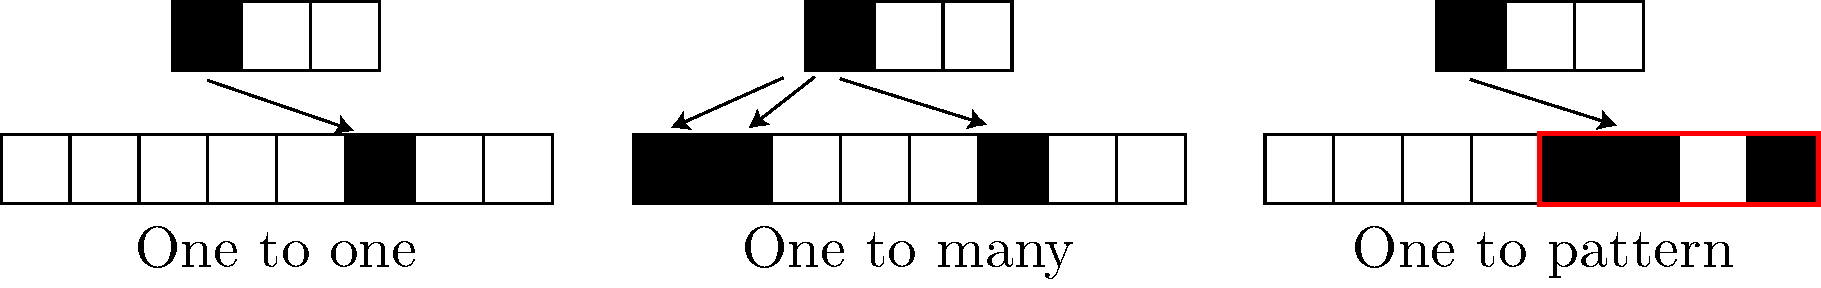
\includegraphics[width=\linewidth]{figures/encoding_methods.pdf}
  \caption{Three encoding methods. From left to right: \emph{one-to-one},
    \emph{one-to-many} and \emph{one-to-pattern}.}\label{fig:enc_meth}
\end{figure}

Following \parencite{yilmazReservoirComputingUsing2014,
  nicheleReservoirComputingUsing2017, nicheleDeepLearningCellular2017}, the
input is projected multiple times to add redundancy to the encoding. This was
experimentally observed to improve performance. We also use a projection vector
larger than the initial one. The projections are randomly generated $R$ times,
applied and concatenated as a single large encoder to create the full CA input
vector. The parameter $R$ is called \emph{redundancy}.

For cellular automata in 1D, the space $\mathcal{P}$ is one-dimensional and the
concatenation is simply done over this dimension. In higher dimensional spaces,
this concatenation has to be defined in some other way.

We write the $R$ projection functions $E_{1}, E_{2}, \ldots, E_{R}$. The
final size of the input vector and the CA state grid is $R \times L_{d}$. We have
\begin{align}
  \vp_{t} = E_{1}(\vx_{t})\mathbin\Vert \ldots \mathbin \Vert E_{R}(\vx_{t})
\end{align}
where $\mathbin\Vert$ is the concatenation operator.

Other projections have been proposed and implemented, for example in
\parencite{yilmazReservoirComputingUsing2014}. We choose to present the three
above because they are simple to understand and implement and their effects can
be explored thoroughly.

\paragraph{Input combination}
There are multiple ways to combine the input vector with the current \ac{CA}
state. \textcite{gloverDynamicalLandscapeReservoir2021} propose to use a XOR
function between the projected input and the \ac{CA} state.

At each input step $t$, the projected input vector $\vp_{t}$ is XORed
element-wise with the current CA state $\vs_{t}$, so that each 1 bit from the
input switches the corresponding bit in the CA state to another value. This
creates a new state $\vs_{t}'$ that the CA will evolve from. $\vs_{t}'$ is
defined as
\begin{align}
  \vs_{t}' \coloneqq \vp_{t} \otimes \vs_{t},
\end{align}
where $\otimes$ is the element-wise XOR operator between two vectors of binary
values, and $\vs'_{t}$ is the temporary CA state resulting from the combination
of the CA state and input vectors at time $t$.

From the \ac{CA} state $\vs'_{t}$, We then compute the next CA states by
applying the update function $\Phi$,

\begin{equation}
  \label{eq:ca-state}
  \vs_{t + 1} = \Phi(\vs'_{t}).
\end{equation}

This is one of many possible ways to combine an input vector with the current
state of the CA that may affect its performance as a reservoir. The XOR-based
input combination gives asymmetrical role to 0 and 1 in the input vectors, which
is natural considering the way we encode and project the categorical data
points. Different cellular automata rules might benefit or get lower performance
because of these encoding choices. The combination problem can be generalized to
incorporate it to the \ac{CA} rule search problem. We demonstrate this in the
next paragraph.

\paragraph{Generalization.} We generalize the input combination method above by
incorporating it to the \ac{CA} update rule. Since the input vector $\vp$ is
binary, we may treat its value at position $i$ as just another virtual \ac{CA}
cell. For an standard \ac{ECA}, the update step takes into account the three
immediate neighbors $\vs^{(i - 1)}, \vs^{(i)}, \vs^{(i + 1)}$ plus the additional
virtual cell $\vp^{(i)}$. Instead of 8 possible input configuration, we now have
16. In this extended \ac{CA} space, the number of possible rules is
$2^{16} = 65536$ instead of 256.

\begin{figure}[htbp]
  \centering
    \begin{subfigure}[b]{.387\linewidth}
    \centering
    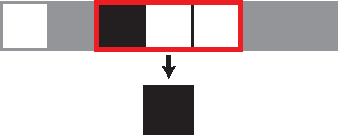
\includegraphics[width=\linewidth]{figures/ca_update_rule.pdf}
    \caption{Regular CA update only takes neighbor states into
      account.}\label{fig:standard-ca-update}
  \end{subfigure}
  \hspace{10pt}
  \begin{subfigure}[b]{.55\linewidth}
    \centering
    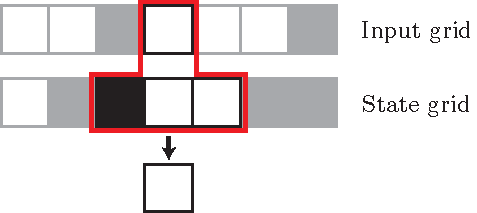
\includegraphics[width=\linewidth]{figures/generalized_ca_update_rule.pdf}
    \caption{The extended neighborhood update also uses an input value to
      decide the next state of a cell.}\label{fig:generalized-ca-update}
  \end{subfigure}
  \caption{Comparison of standard CA update rule and our extended input
    combination rule.\label{fig:ca_update_rule}}
\end{figure}

This method is illustrated in Fig.~\ref{fig:ca_update_rule} along the regular CA
update. It generalizes the concept of input combination with the state $\vs$.
The XOR method described above is one of its special cases, but our method also
contains all the possible boolean function with 4 inputs.

\paragraph{Building the reservoir}
The final reservoir state $\vr_{t + 1}$ is obtained by concatenating $r$
consecutive CA states obtained from a single combined state $\vs'$ by applying
$\Phi$ again. If the size of the state is $n$, the resulting reservoir vector
$\vr$ has a dimension $K = r \times n$, where $r$ is defined above. As for the
\ac{ESN}, the $L$-dimensional output tokens are calculated at times $t > 0$ as
$\tilde{\vx}_{t+ 1} = D(\vr_{t})$ where
$D: \mathbb{R}^{K} \rightarrow \mathbb{R}^{L}$ is the (trained) decoding
function. Usually a linear decoding function is used, such that
$D(\vr_{t}) = \mW_{\text{out}}\vr_{t}$. The complete process of \ac{RC} with
\ac{CA} is summarized in figure \ref{fig:reca-schema}.

\begin{figure}[htbp]
  \centering
  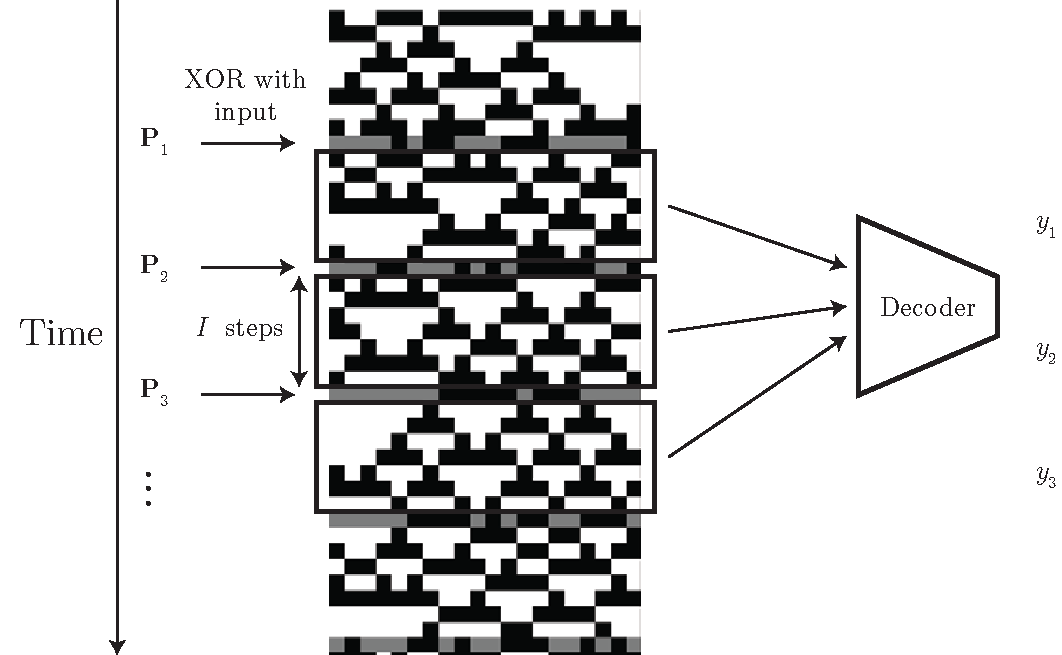
\includegraphics[width=.6\linewidth]{figures/reca_schema.pdf}
  \caption{Global illustration of the ReCA model with the XOR-based input and
    state combinationmethod .}\label{fig:reca-schema}
\end{figure}
